\subsubsection{\stid{1.14} GASNet-EX}
\paragraph{Overview} 

The Lightweight Communication and Global Address Space Support project (Pagoda)
is developing GASNet-EX, a portable high-performance communication layer
supporting multiple implementations of the Partitioned Global Address Space
(PGAS) model.
GASNet-EX clients include Pagoda's PGAS programming interface UPC++~\cite{Bachan:paw17,upcxx-site}
 and the Legion Programming
System~\cite{bauer2012legion,legion-site} (WBS~2.3.1.08).

GASNet-EX's low-overhead communication mechanisms are designed to maximize
injection rate and network utilization, tolerate latency through
overlap, streamline unpredictable communication events, minimize
synchronization, and efficiently support small- to medium-sized
messages arising in ECP applications.  GASNet-EX enables the ECP
software stack to exploit the best-available communication mechanisms,
including novel features still under development by vendors.  The
GASNet-EX communications library and the PGAS models built upon it
offer a complementary, yet interoperable, approach to MPI with OpenMP,
enabling developers to focus their effort on optimizing
performance-critical communication.

We are co-designing GASNet-EX with the UPC++ development team with
additional input from the Legion and
(non-ECP) Cray Chapel~\cite{chapel-chapter,chapel-site} projects.

\paragraph{Key  Challenges}

Exascale systems will deliver exponential growth in on-chip parallelism and
reduced memory capacity per core, 
increasing the importance of strong
scaling and finer-grained communication events.  
Success at Exascale demands that
software needs to minimize the work performed by lightweight cores and avoid the
overhead of long, branchy serial code paths; 
this motivates a requirement for efficient
fine-grained communication.
These problems are exacerbated by application trends; many of the ECP applications require
adaptive meshes, sparse matrices,
or dynamic load balancing.
All of these characteristics favor the use of
low-overhead communication mechanisms that
can maximize injection rate and network utilization, tolerate latency through
overlap, accommodate unpredictable communication events, minimize synchronization,
and efficiently support small- to medium-sized messages. The ECP software stack
needs to expose the best-available communication mechanisms, including novel
features being developed by the vendor community.

\paragraph{Solution Strategy}

The PGAS model is a powerful means of addressing these
challenges and is critical in building other ECP programming systems,
libraries, and applications.  We use the term {\em PGAS} for models that support
one-sided communication, 
including contiguous and non-contiguous remote memory access (RMA) operations such as put/get
and atomic updates). Some of these models also include support for remote function invocation.
GASNet-EX is a communications library that provides the foundation for implementing
PGAS models, and is the successor to the widely-deployed GASNet library.
We are building on 15 years of experience with the GASNet~\cite{gasnet-spec,gasnet-site}
communication layer to provide production-quality implementations that include
improvements motivated by
technology trends and application experience.  

The goal of the GASNet-EX work is to provide a portable, high-performance GAS
communication layer for Exascale and pre-Exascale systems, addressing the challenges
identified above.
GASNet-EX provides interfaces that efficiently match the RDMA capabilities of modern
inter-node network hardware and intra-node communication between distinct address spaces.
Interfaces for atomics and collectives are being developed to enable offload to current
and future network hardware with corresponding capabilities.
These design choices and their implementations supply the low-overhead communications
mechanisms required to address the requirements of Exascale applications.


\paragraph{Recent Progress}

Work on GASNet-EX to date has consisted of introducing new capabilities and
selective performance tuning of those capabilities. 

Two new capabilities, ``Collectives'' and ``Non-Contiguous RMA
(VIS)'', update and formalize features which existed as experimental
extensions to GASNet-1.  Updates to the Collectives APIs relative to the
GASNet-1 design enable offload to appropriate network hardware.  Updates to the
Non-Contiguous RMA APIs include the ability to express transposes and
reflections, as well as a ``Dependent Operations'' capability to execute a
``Peer Completion Handler'' at the end of a transfer.

Capabilities entirely new to GASNet-EX include ``Negotiated-Payload Active
Messages'', ``Immediate Operations'', ``Local Completion'' and ``Remote
Atomics''.  GASNet-EX contains ``reference'' implementations of these features
in terms of the pre-existing GASNet-EX functionality, available on all
networks.  While these reference implementations are correct and functionally
complete, they do not take advantage of network-specific mechanisms.
Network-specific implementations (``specializations'') of these features for
the Cray Aries network (used in Cray XC-series systems) have shown significant
performance gains over the reference implementations ~\cite{gasnet-aries}.
%
Most notably, offload of atomics to the Aries NIC yields a 1.7x latency improvement
and greatly benefits scalability in a many-to-one atomics hot-spot
test.

The addition of ``Subset Teams'' support to all GASNet-EX communications APIs
provides the means to name communication peers using subset-scoped ranks and
enables the use of Collectives over subsets.


\begin{figure}[htb]
  \centering
  \subfloat[8-byte RMA Latencies\label{fig:rma-lat-bars}]{
     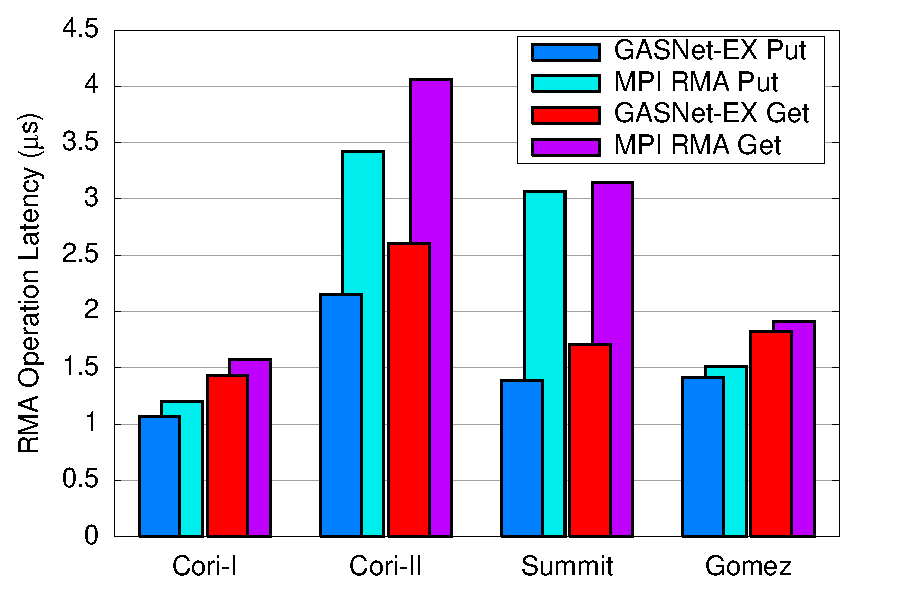
\includegraphics[width=0.432\textwidth]{projects/2.3.1-PMR/2.3.1.14-UPCxx-GASNet/latency_bars.pdf}
  }
  \subfloat[Aries Flood Bandwidth\label{fig:cori1-bw}]{
     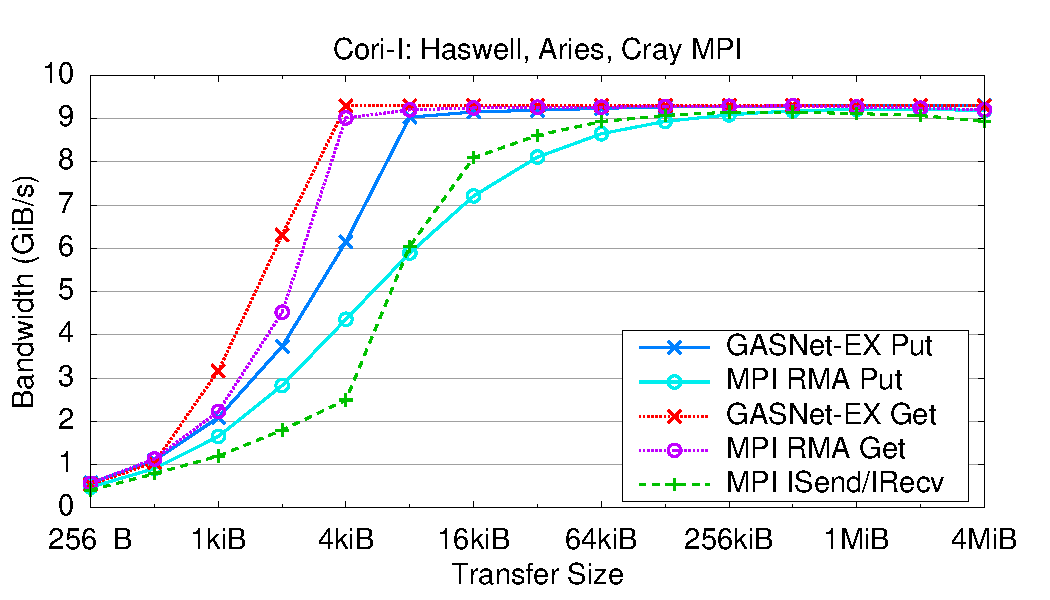
\includegraphics[width=0.504\textwidth]{projects/2.3.1-PMR/2.3.1.14-UPCxx-GASNet/CoriHSW-slide-BW.pdf}
  }
  \caption{\label{fig:gasnet-ex-rma} Selected GASNet-EX vs. MPI RMA Performance Results}
\end{figure}

The addition of new capabilities to GASNet-EX has not come at the expense of
performance.
Figure~\ref{fig:gasnet-ex-rma} shows representative results from a
recent paper~\cite{gasnet-lcpc18} comparing
the RMA performance of GASNet-EX with MPI on multiple systems including
NERSC's Cori and OLCF's Summitdev%
\footnote{The paper's results from Summitdev
have been replaced by more recent (Nov 8, 2018) results from OLCF's newer Summit system.  The authors
gratefully acknowledge the assistance of Geoffroy Vall\'ee of ORNL, who
collected the results on Summit.}.
%
The paper presents experimental methodology and system descriptions, which are
also available online~\cite{gasnet-site}, along with results for additional
systems.

Figure~\ref{fig:rma-lat-bars} shows the latency of 8-byte RMA Put and Get operations on
four systems, including two distinct networks and three distinct MPI
implementations.
%
GASNet-EX's latency is 6\% to 55\% better than MPI's on Put and 5\% to 45\%
better on Get.
%
Algorithms sensitive to small-transfer latency become practical in PGAS
programming models due to these improvements relative to MPI.

Figure~\ref{fig:cori1-bw} shows flood bandwidth of RMA Put and Get on Cori
Phase~I.  GASNet-EX's bandwidth is seen to rise to saturation at smaller
transfer sizes than Cray MPI, with the most pronounced differences
appearing in the 512 to 8192 byte range.
%
Comparison to the bandwidth of MPI message-passing (green series) illustrates the
benefits of one-sided communication, a major feature of PGAS models.

\paragraph{Next Steps}

Our next efforts include:
\begin{enumerate}

\item \textbf{Multiple Endpoints and Segments}.  Support for multiple
communications endpoints and multiple memory segments will provide immediate
benefit to multi-threaded runtimes by reducing contention for shared resources.
Additionally, these features enable future work on hardware offload of
transfers to and from GPU memories (\textit{e.g.} use of GPUDirect).

\item \textbf{Specialization for InfiniBand}.  Network-specific implementations
of new GASNet-EX features for the InfiniBand network will provide performance
benefits on systems such as OLCF's Summit.  The benefits of such specialization
for the Cray Aries network has been demonstrated previously~\cite{gasnet-aries}.

\item \textbf{Client-Driven Tuning}.  In collaboration with authors of client
runtimes using GASNet-EX (most notably UPC++ and Legion), any significant
bottlenecks or performance anomalies will be identified and addressed.

\end{enumerate}
